\chapter{Introduction}
\label{Chapter:Intro}

This .pdf was rendered by the main .tex file, Thesis.tex. This file is formatted primarily by the document class `UIdaho', which is provided by ./rcs/uidaho.cls. Thesis.tex contains very little of the text that makes up this template. Instead, it inputs files for each chapter. For a document as large as a thesis or dissertation usually ends up being, this makes keeping track of everything a lot easier. The text for the frontmatter (everything before this chapter) is contained in the folder ./Frontmatter/. Each of the chapters are contained in ./Chapters/, and the appendices are contained in ./Appendix/. This chapter, \cref{Chapter:Intro}, can be found at ./Chapters/Introduction.tex, and will tell you how to change the template into your thesis.

\section{Cover Page}\label{Section:Intro-Cover}
The first thing you need to do is update your cover page. This is done in Thesis.tex, by updating the `Thesis Information', as shown by \cref{Fig:CoverPage}. This information is populated to form the cover page by the \verb|\thesistitlepage| macro. If you are a Ph.D student, be sure to change the \verb|\doctype| and \verb|\thesisdegree|.

\begin{figure}[h!]
    \centering
    
\includegraphics[width = 0.5\textwidth]{CoverpageInfo}
    \caption[Cover Page Info]{Change the cover page info in this section of Thesis.tex. This information is automatically populated by the UIdaho document class.}
    \label{Fig:CoverPage}
\end{figure}

\section{MetaData}
\label{Section:Intro-MetaData}

The next thing to do is to update your .pdf metadata. This is done by updating the fields displayed by \cref{Fig:MetaData}

\begin{figure}[h!]
    \centering
    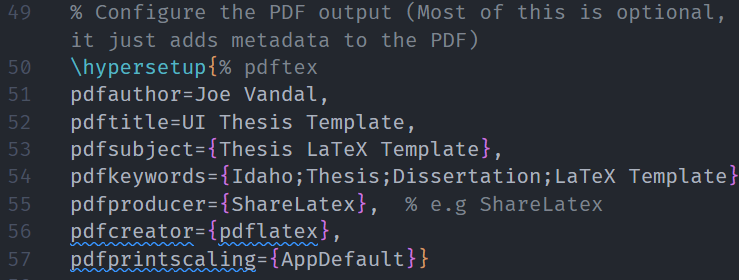
\includegraphics[width = 0.5\textwidth]{MetaData}
    \caption[MetaData]{Change the information in this section of Thesis.tex. This information tells the pdf reader what to display as the document title, among other things.}
    \label{Fig:MetaData}
\end{figure}

\section{Everything Else}
\label{Section:Intro-Else}

Now, its as simple as writing your abstract, acknowledgements, dedication, statement of contribution (if applicable), your chapters, and any appendices you may choose to include. Good luck! 